\documentclass[9pt,aspectratio=169,xcolor=table]{beamer}

%~~~~~~~~~~~~~~~~~~~~~~~~~~~~~~~~~~~~~~~~~~~~~~~~~~~~~~~~~~~~~~~~~~~~~~~~~~~~~~
% Use roboto Font (recommended)
\usepackage[sfdefault]{roboto}
\usepackage[utf8]{inputenc}
\usepackage[T1]{fontenc}
%~~~~~~~~~~~~~~~~~~~~~~~~~~~~~~~~~~~~~~~~~~~~~~~~~~~~~~~~~~~~~~~~~~~~~~~~~~~~~~

%~~~~~~~~~~~~~~~~~~~~~~~~~~~~~~~~~~~~~~~~~~~~~~~~~~~~~~~~~~~~~~~~~~~~~~~~~~~~~~
% Define where theme files are located. ('/styles')
\usepackage{styles/fluxmacros}
\usefolder{styles}
% Use Flux theme v0.1 beta
% Available style: asphalt, blue, red, green, gray
\usetheme[style=hunter]{flux}
%~~~~~~~~~~~~~~~~~~~~~~~~~~~~~~~~~~~~~~~~~~~~~~~~~~~~~~~~~~~~~~~~~~~~~~~~~~~~~~

%~~~~~~~~~~~~~~~~~~~~~~~~~~~~~~~~~~~~~~~~~~~~~~~~~~~~~~~~~~~~~~~~~~~~~~~~~~~~~~
% Extra packages
\usepackage{booktabs}
\usepackage{colortbl}
\usepackage{ragged2e}
\usepackage{amssymb}
\usepackage{multirow}
\usepackage{tikz}
\usetikzlibrary{arrows.meta, positioning, fit, backgrounds, calc, decorations.pathreplacing}
\setbeamertemplate{itemize items}[square]
\usepackage[scaled=.8]{beramono}
\usepackage{listings}
\usepackage{styles/lstlangarm}
\usepackage{array}
\usepackage{makecell}
\definecolor{bgcolor}{HTML}{F2E9E9}
% lstlangarm.sty references \color{mauve} for string literals but never defines
% it -- only fires when a listing contains a string. Define it here.
\definecolor{mauve}{rgb}{0.58,0,0.82}
% lstlangarm's C style sets commentstyle=green!20, which is unreadable on the
% pink listing background. Darken it globally.
\lstset{commentstyle=\color{green!45!black}}
% ragged-right fixed-width column -- must be defined in the preamble, never
% inside a frame (\newcolumntype's #1 breaks beamer's frame scanner)
\newcolumntype{R}[1]{>{\RaggedRight\arraybackslash}p{#1}}
%~~~~~~~~~~~~~~~~~~~~~~~~~~~~~~~~~~~~~~~~~~~~~~~~~~~~~~~~~~~~~~~~~~~~~~~~~~~~~~
% Table striping: odd rows white, even rows very light gray.
% Needs \documentclass[...,xcolor=table]{beamer} (beamer loads xcolor itself,
% so the option must go on the class, not \usepackage).
\definecolor{stripe}{gray}{0.94}
% \striped makes body rows alternate white, gray, white, ... starting white.
% \rowcolors counts from the first coloured body row; the header is not counted.
\newcommand{\striped}{\rowcolors{1}{white}{stripe}}
%~~~~~~~~~~~~~~~~~~~~~~~~~~~~~~~~~~~~~~~~~~~~~~~~~~~~~~~~~~~~~~~~~~~~~~~~~~~~~~

%~~~~~~~~~~~~~~~~~~~~~~~~~~~~~~~~~~~~~~~~~~~~~~~~~~~~~~~~~~~~~~~~~~~~~~~~~~~~~~
% TikZ block styles -- matches ch1/ch2
% Colour variables are named identically in the book's stm32primer.tex, so any
% tikzpicture using only the \tikzset{...} styles below can be copied verbatim
% between slides and book. Only the \definecolor/\colorlet VALUES differ: the
% book is printed, so it keeps every stroke pure black with muted fills. These
% slides are projected, so both fill AND stroke are bright and saturated to
% grab attention -- see stm32primer.tex for the print palette.
\definecolor{blkfill}{HTML}{DDEEDD}
\definecolor{blkline}{HTML}{355E3B}
\definecolor{accentfill}{HTML}{FFE0B2}
\definecolor{accentline}{HTML}{E65100}
\definecolor{memfill}{HTML}{DFF5DA}
\definecolor{memline}{HTML}{2E7D32}
\definecolor{cellfill}{HTML}{FFFFFF}
\definecolor{cellline}{HTML}{424242}
\definecolor{bitmaskfill}{HTML}{DCEBFF}
\definecolor{bitmaskline}{HTML}{1565C0}
\definecolor{bithitfill}{HTML}{FFE0B2}
\definecolor{bithitline}{HTML}{E65100}
\tikzset{
  blk/.style   = {rectangle, rounded corners=2pt, draw=blkline, fill=blkfill,
                  thick, align=center, font=\small, minimum height=9mm, inner sep=3pt},
  cpublk/.style= {rectangle, rounded corners=2pt, draw=accentline, fill=accentfill,
                  thick, align=center, font=\small\bfseries, minimum height=9mm, inner sep=3pt},
  memblk/.style= {rectangle, rounded corners=2pt, draw=memline, fill=memfill,
                  thick, align=center, font=\small, minimum height=9mm, inner sep=3pt},
  cell/.style  = {rectangle, draw=cellline, fill=cellfill, align=center,
                  font=\small\ttfamily, minimum height=7mm, inner sep=2pt},
  bitcell/.style={rectangle, draw=cellline, fill=cellfill, thick,
                  minimum width=5.4mm, minimum height=5.4mm, inner sep=0pt,
                  font=\scriptsize\ttfamily, anchor=center},
  bitmask/.style={bitcell, fill=bitmaskfill, draw=bitmaskline},
  bithit/.style ={bitcell, fill=bithitfill, draw=bithitline, font=\scriptsize\ttfamily\bfseries},
  rowlab/.style ={font=\scriptsize, text=Gray, anchor=east},
  oplab/.style  ={font=\scriptsize\itshape, text=Gray, anchor=west},
  lbl/.style   = {font=\scriptsize, text=Gray},
  flow/.style  = {-{Stealth[length=2mm]}, thick, draw=blkline},
  busline/.style={thick, draw=cellline},
}
% NOTE (theme quirks -- all fail SILENTLY, always page through the PDF):
%  - a second \\ inside a nested {...} group in a TikZ node breaks parsing
%  - {\small ...} wrapped around a nested itemize eats the frame title + list
%  - \usebeamercolor on a [plain] frame falls through to an unstyled default
%  - \newcolumntype inside a frame breaks beamer's frame scanner
%  - lstlisting needs \begin{frame}[fragile]
%  - a TikZ picture wider than its column silently overflows into neighbours
%~~~~~~~~~~~~~~~~~~~~~~~~~~~~~~~~~~~~~~~~~~~~~~~~~~~~~~~~~~~~~~~~~~~~~~~~~~~~~~

%%%%%%%%%%%%%%%%%%%%%%%%%%%%%%%%%%%
%% BEGIN CONDITIONAL COMPILATION %%
%%%%%%%%%%%%%%%%%%%%%%%%%%%%%%%%%%%
\newif\ifwebex
%\webextrue % uncomment to generate section separator
\ifwebex
\AtBeginSection[]{
  \begin{frame}
  \vfill
  \centering
  \begin{beamercolorbox}[sep=8pt,center,shadow=true,rounded=true]{title}
    \usebeamerfont{title}\insertsectionhead\par%
  \end{beamercolorbox}
  \vfill
  \end{frame}
}
\else
\AtBeginSection[]
{
{
    \setbeamercolor{background canvas}{bg=yellow!10}
    \begin{frame}[plain]
        \frametitle{Table of Contents}
        \tableofcontents[currentsection]
    \end{frame}
}
}
\fi
%%%%%%%%%%%%%%%%%%%%%%%%%%%%%%%%%%%
%% END CONDITIONAL COMPILATION   %%
%%%%%%%%%%%%%%%%%%%%%%%%%%%%%%%%%%%

%~~~~~~~~~~~~~~~~~~~~~~~~~~~~~~~~~~~~~~~~~~~~~~~~~~~~~~~~~~~~~~~~~~~~~~~~~~~~~~
% Information
\title{FSM Analysis}
\subtitle{\emph{Contemporary Digital Electronic Systems} --- Chapter 14}
\author{Mun\'{i}m Zabidi}
\institute{\color{primary}Faculty of Electrical Engineering, Universiti Teknologi Malaysia}
\date{\today}
\titlegraphic{assets/logoutmwhite.png}
\graphicspath{{.}{../fig/}}
%~~~~~~~~~~~~~~~~~~~~~~~~~~~~~~~~~~~~~~~~~~~~~~~~~~~~~~~~~~~~~~~~~~~~~~~~~~~~~~

\newcommand{\figh}[2]{\includegraphics[height=#1\textheight]{#2}}



\begin{document}

\titlepage

%===============================================================================
\section{Why This Chapter}
%===============================================================================

\begin{frame}{Why This Chapter Matters}
  \begin{columns}[c]
  \begin{column}{.47\textwidth}
    Design goes from specification to circuit; analysis goes the other way. Given a sequential schematic, can you recover the \alert{state diagram} and the behaviour? That is how you document legacy circuits, debug someone else's design, and verify your own.
  \end{column}
  \begin{column}{.51\textwidth}
    \begin{block}{After this chapter, you can:}
    {\small
    \begin{enumerate}\itemsep2pt
      \item Identify the state register and the next-state and output logic in a schematic.
      \item Derive the flip-flop input and output equations by inspection.
      \item Build the state table from those equations.
      \item Draw the state diagram from the state table.
      \item Classify the recovered FSM as Moore or Mealy.
    \end{enumerate}}
    \end{block}
  \end{column}
  \end{columns}
\end{frame}

\begin{frame}{An Opening Question}
  \leavevmode\vspace{4mm}
  \begin{center}
  \fbox{\parbox{.78\textwidth}{\centering\vspace{2mm}
  \large If you were handed an unlabelled chip containing a small FSM, what would you do to reconstruct its \alert{state diagram}?
  \vspace{2mm}}}
  \end{center}
  \vspace{4mm}
  This chapter does it from the schematic, which is the same job on paper.
\end{frame}

%===============================================================================
\section{The Analysis Procedure}
%===============================================================================

\begin{frame}{Reverse Engineering an FSM}
  \begin{columns}[c]
  \begin{column}{.5\textwidth}
    \begin{itemize}\small\itemsep3pt
      \item Analysis is \alert{reverse engineering}: understand a system from its structure and operation.
      \item Needed when a legacy circuit must be rebuilt (parts discontinued, documentation lost), to understand undocumented designs, to estimate cost and find improvements, even to assess patent infringement.
    \end{itemize}
  \end{column}
  \begin{column}{.48\textwidth}
    \centering
    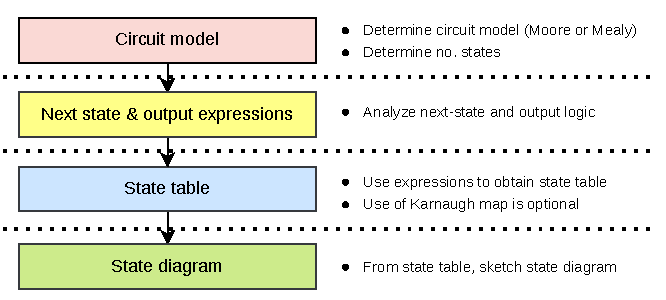
\includegraphics[width=\textwidth]{fsm_analysis}
  \end{column}
  \end{columns}
  \begin{enumerate}\small\itemsep2pt
    \item Identify the model (Moore or Mealy) and the number of states.
    \item Derive the next-state and output expressions.
    \item Build the state table (K-maps optional).
    \item Draw the state diagram.
  \end{enumerate}
\end{frame}

%===============================================================================
\section{Moore Machine}
%===============================================================================

\begin{frame}{Moore Circuit: Steps 1 and 2}
  \begin{columns}[c]
  \begin{column}{.45\textwidth}
    \centering
    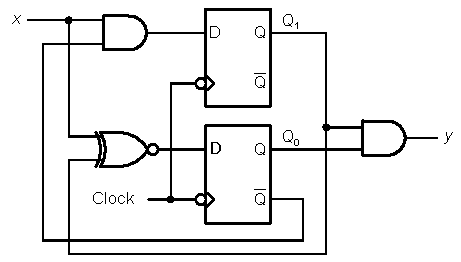
\includegraphics[width=\textwidth]{analyzemoore_sc}
  \end{column}
  \begin{column}{.53\textwidth}
    \begin{block}{Step 1: model and number of states}
      \small Output $y$ comes only from flip-flop outputs, with no direct path from $x$: \alert{Moore}. Two flip-flops: up to 4 states.
    \end{block}
    \begin{block}{Step 2: equations}
      \small
      $D_1 = Q_0'x \qquad D_0 = \overline{Q_1 \oplus x} = Q_1x + Q_1'x'$\\
      D flip-flops: $Q^+ = D$, so these are the next-state equations.\\
      $y = Q_1Q_0$
    \end{block}
  \end{column}
  \end{columns}
\end{frame}

\begin{frame}{Moore Circuit: Minterms}
  \begin{columns}[c]
  \begin{column}{.52\textwidth}
    \small Canonical SOP route (indices $Q_1Q_0x$):
    \begin{align*}
      Q_1^+ &= Q_0'x = Q_1'Q_0'x + Q_1Q_0'x = \textstyle\sum m(1,5) \\
      Q_0^+ &= Q_1x + Q_1'x' = \textstyle\sum m(0,2,5,7)
    \end{align*}
  \end{column}
  \begin{column}{.46\textwidth}
    \centering
    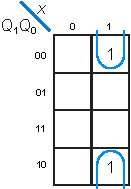
\includegraphics[height=.22\textheight]{analyzemoore_kmap1}\hspace{1mm}
    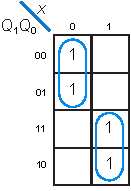
\includegraphics[height=.22\textheight]{analyzemoore_kmap2}\hspace{1mm}
    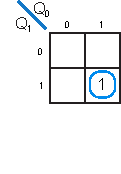
\includegraphics[height=.22\textheight]{analyzemoore_kmap3}\\[1mm]
    {\scriptsize $Q_1^+$ \hspace{.12\textwidth} $Q_0^+$ \hspace{.12\textwidth} $y$}
  \end{column}
  \end{columns}
  \begin{itemize}\small
    \item Either the K-map or the canonical-SOP route gives the same state table.
  \end{itemize}
\end{frame}

\begin{frame}{Moore Circuit: State Table and Diagram}
  \begin{columns}[c]
  \begin{column}{.45\textwidth}
    \centering\small\striped
    \begin{tabular}{@{}cc|cc@{}}
      \toprule
      $Q_1Q_0$ & $x$ & $Q_1^+Q_0^+$ & $y$ \\
      \midrule
      00&0&01&0 \\ 00&1&10&0 \\ 01&0&01&0 \\ 01&1&00&0 \\
      10&0&00&0 \\ 10&1&11&0 \\ 11&0&00&1 \\ 11&1&01&1 \\
      \bottomrule
    \end{tabular}
  \end{column}
  \begin{column}{.53\textwidth}
    \centering
    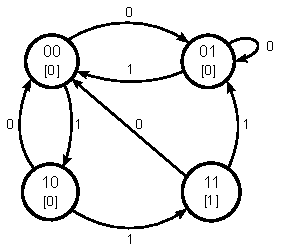
\includegraphics[height=.45\textheight]{analyzemoore_sd}
    \begin{itemize}\small
      \item Step 4: each table row becomes an arrow; the output sits inside each state.
    \end{itemize}
  \end{column}
  \end{columns}
\end{frame}

%===============================================================================
\section{Mealy Machine}
%===============================================================================

\begin{frame}{Mealy Circuit}
  \begin{columns}[c]
  \begin{column}{.45\textwidth}
    \centering
    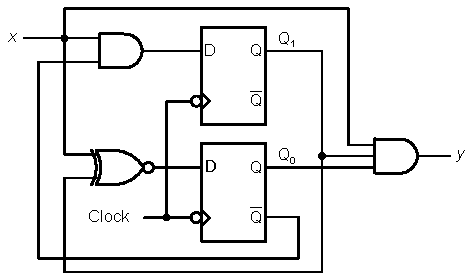
\includegraphics[width=\textwidth]{analyzemealy_sc}
  \end{column}
  \begin{column}{.53\textwidth}
    \begin{block}{Steps 1 and 2}
      \small The input $x$ goes straight to the rightmost AND gate: \alert{Mealy}. Two flip-flops: $2^2 = 4$ states.\\[1mm]
      $Q_1^+ = D_1 = Q_0'x$\\
      $Q_0^+ = D_0 = Q_1x + Q_1'x'$\\
      $y = Q_1Q_0x$
    \end{block}
  \end{column}
  \end{columns}
\end{frame}

\begin{frame}{Mealy Circuit: State Table from a K-Map}
  \begin{columns}[c]
  \begin{column}{.52\textwidth}
    \centering
    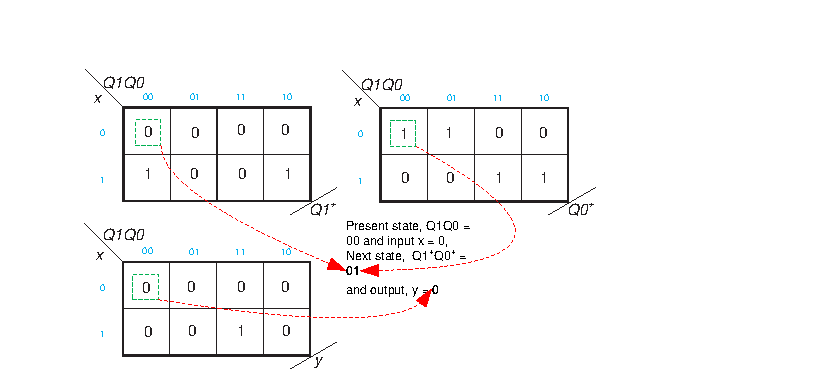
\includegraphics[width=\textwidth]{kmap_analyze_mealy_simple}
  \end{column}
  \begin{column}{.46\textwidth}
    \begin{itemize}\small\itemsep3pt
      \item Lay out a K-map whose inputs are the present state $Q_1Q_0$ and $x$.
      \item Fill each cell with the next state $Q_1^+Q_0^+$ and output $y$.
      \item Each cell is one arrow of the state diagram.
    \end{itemize}
    \centering
    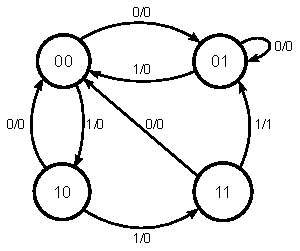
\includegraphics[height=.3\textheight]{analyzemealy_sd}
  \end{column}
  \end{columns}
\end{frame}

\begin{frame}{Moore versus Mealy Waveforms}
  \centering
  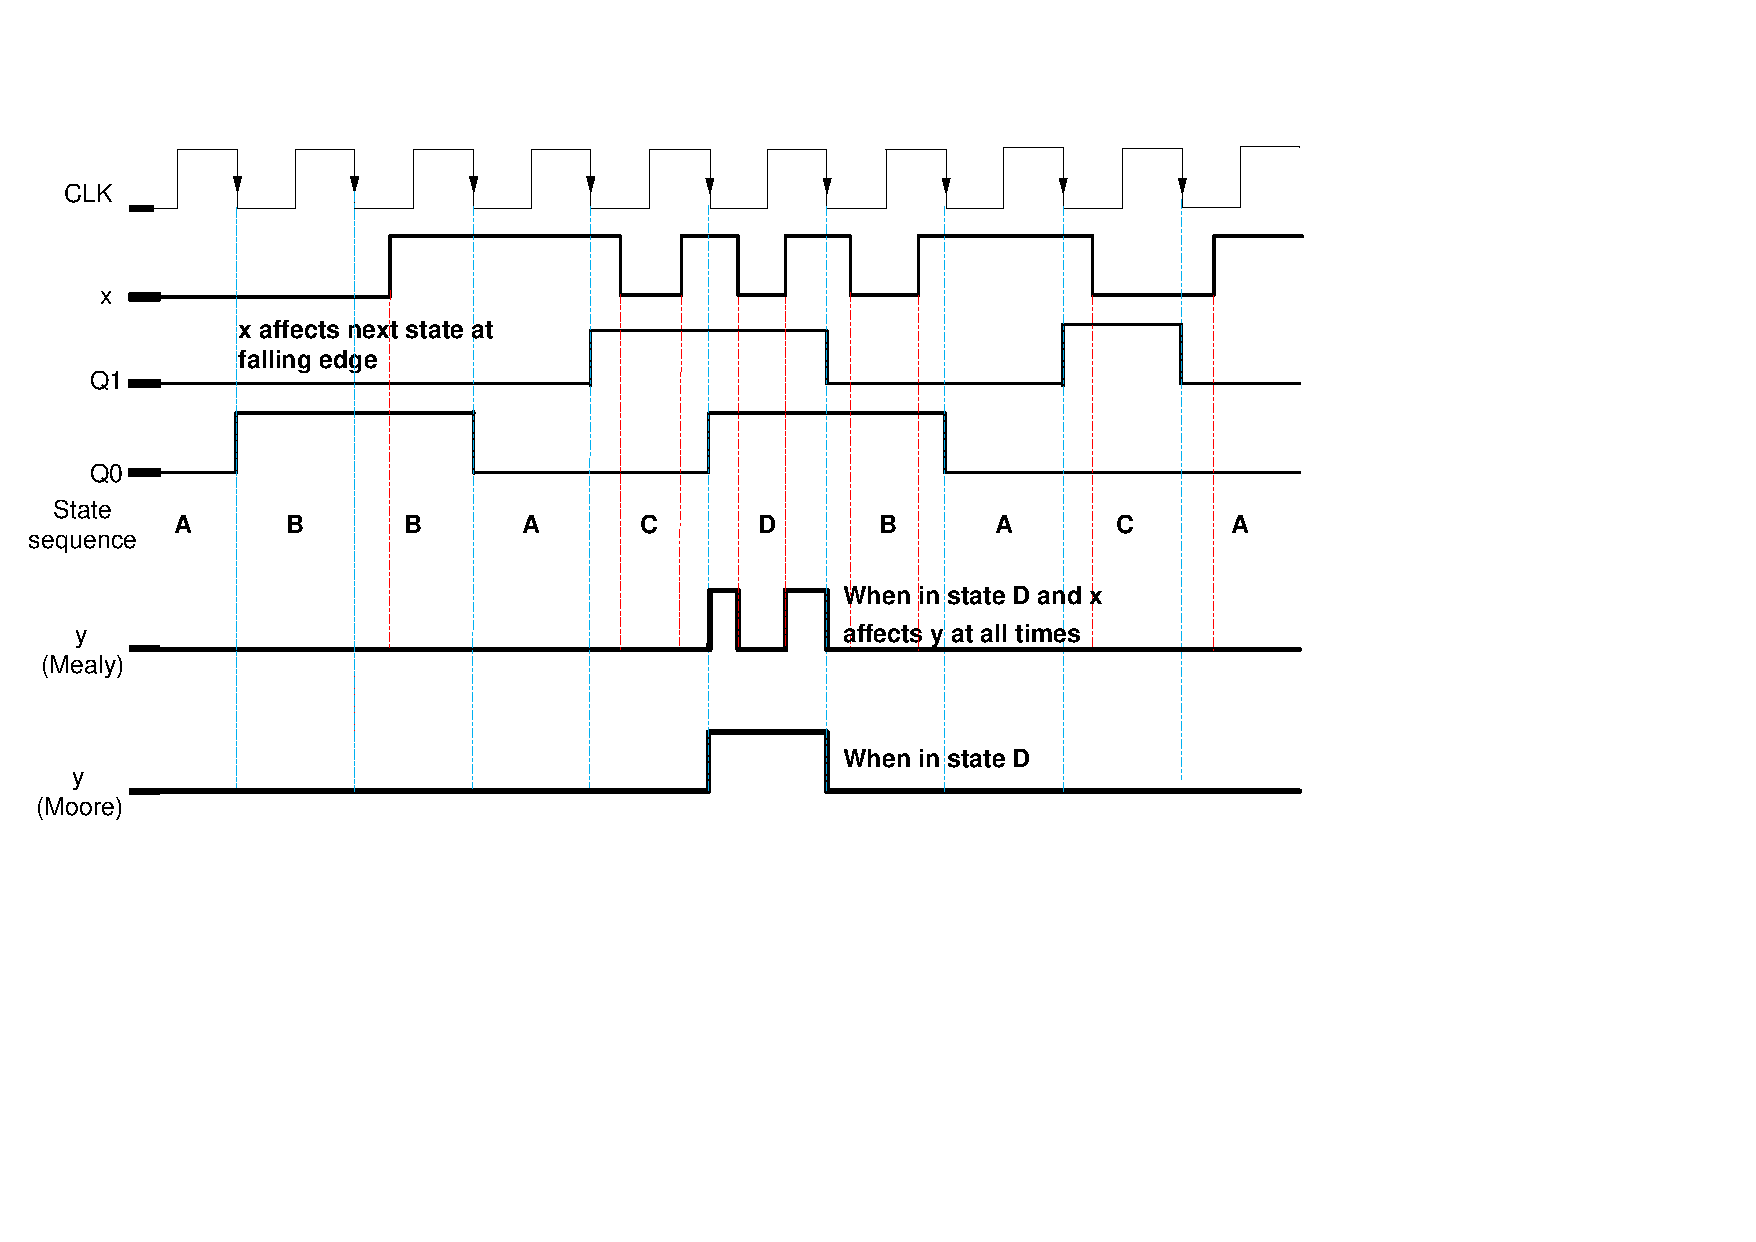
\includegraphics[height=.5\textheight]{wvf_analyze_moore_mealy_simple}
  \begin{itemize}\small\itemsep2pt
    \item A waveform can replace a state diagram for showing next state and output.
    \item The Moore output changes synchronously with the clock edge.
    \item The Mealy output can glitch: the asynchronous input $x$ changes it immediately, whatever the clock does.
  \end{itemize}
\end{frame}

%===============================================================================
\section{JK Flip-Flop FSM}
%===============================================================================

\begin{frame}{Analysing a JK-Based Circuit}
  \begin{columns}[c]
  \begin{column}{.4\textwidth}
    \centering
    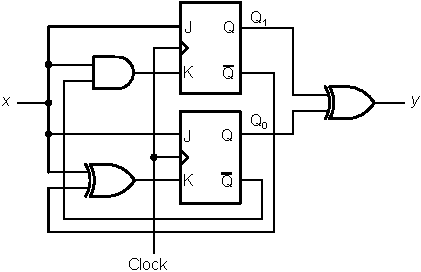
\includegraphics[width=\textwidth]{analyzejk_sc}
  \end{column}
  \begin{column}{.58\textwidth}
    \begin{itemize}\small\itemsep3pt
      \item JK flip-flops are not recommended for new designs, but legacy TTL circuits still use them.
      \item Step 1: the output depends only on the state: \alert{Moore}; $2^2 = 4$ states.
      \item Step 2: flip-flop inputs $J_1 = x$, $K_1 = Q_0'x$, $J_0 = x$, $K_0 = Q_1'\oplus x$; output $y = Q_1 \oplus Q_0$.
    \end{itemize}
  \end{column}
  \end{columns}
\end{frame}

\begin{frame}{JK Circuit: Next-State Equations}
  \begin{itemize}\small\itemsep3pt
    \item Substitute into the JK characteristic equation $Q^+ = JQ' + K'Q$.
  \end{itemize}
  \small
  \begin{align*}
    Q_1^+ &= xQ_1' + (Q_0'x)'Q_1 = Q_1'x + Q_1Q_0 + Q_1x' = \textstyle\sum m(1,3,4,6,7) \\
    Q_0^+ &= xQ_0' + (Q_1'\oplus x)'Q_0 = Q_0'x + Q_1'Q_0x + Q_1Q_0x' = \textstyle\sum m(1,3,5,6)
  \end{align*}
  \begin{block}{Unlike the D flip-flop}
    \small For a JK flip-flop the input equations are \emph{not} the next-state equations: always apply the characteristic equation.
  \end{block}
\end{frame}

\begin{frame}{JK Circuit: State Table and Diagram}
  \begin{columns}[c]
  \begin{column}{.45\textwidth}
    \centering\small\striped
    \begin{tabular}{@{}cc|cc@{}}
      \toprule
      $Q_1Q_0$ & $x$ & $Q_1^+Q_0^+$ & $y$ \\
      \midrule
      00&0&00&0 \\ 00&1&11&0 \\ 01&0&00&1 \\ 01&1&11&1 \\
      10&0&10&1 \\ 10&1&01&1 \\ 11&0&11&0 \\ 11&1&10&0 \\
      \bottomrule
    \end{tabular}
  \end{column}
  \begin{column}{.53\textwidth}
    \centering
    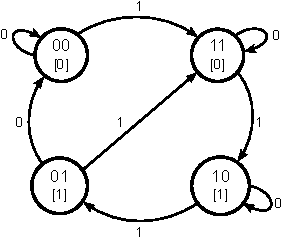
\includegraphics[height=.45\textheight]{analyzejk_sd}
  \end{column}
  \end{columns}
\end{frame}

\begin{frame}{Back to the Opening Question}
  \begin{block}{Reconstructing the state diagram}
    \small For a real chip you would probe the flip-flop outputs and the output pins while applying input patterns, and record, for each present state and input, the next state and output: you would be building the \alert{state table} directly. This chapter does the same on paper, with the equations read off the schematic, so the table can be filled in exhaustively.
  \end{block}
\end{frame}

%===============================================================================
\section{Summary}
%===============================================================================

\begin{frame}{Summary}
  \begin{itemize}\itemsep3pt\small
    \item D flip-flop circuits are the easiest to analyse: $Q^+ = D$, so the input equations are also the next-state equations.
    \item For JK flip-flops, use the characteristic equation to convert input equations into next-state equations.
    \item Enumerate every (state, input) pair to fill the state table; read the state diagram from it.
    \item A direct path from an input to an output means Mealy; otherwise Moore.
  \end{itemize}
  \begin{block}{Looking ahead}
    Chapter 15 scales the design procedure up to controllers: FSMs with several inputs and outputs that drive the rest of a system.
  \end{block}
\end{frame}

\end{document}
